\documentclass[aspectratio=169,10pt]{beamer}

% ---- Packages ----------------------------------------------------------
\usepackage[T1]{fontenc}
\usepackage{lmodern}
\usepackage{microtype}
\usepackage{booktabs}
\usepackage{array}
\usepackage{multirow}
\usepackage{graphicx}
\usepackage{tikz}
\usepackage{xcolor}
\usepackage{amsmath}
\usepackage{calc}

\graphicspath{{../preprocessing_report/figures/}}

% ---- Brand palette -----------------------------------------------------
\definecolor{garnet}{HTML}{73000A}
\definecolor{rose}{HTML}{CC2E40}
\definecolor{atlantic}{HTML}{466A9F}
\definecolor{congaree}{HTML}{1F414D}
\definecolor{horseshoe}{HTML}{65780B}
\definecolor{honeycomb}{HTML}{A49137}
\definecolor{warmgrey}{HTML}{676156}
\definecolor{sandstorm}{HTML}{FFF2E3}
\definecolor{black90}{HTML}{363636}
\definecolor{black70}{HTML}{5C5C5C}
\definecolor{black50}{HTML}{A2A2A2}
\definecolor{black30}{HTML}{C7C7C7}
\definecolor{black10}{HTML}{ECECEC}

% ---- Theme: flat, no rounded edges -------------------------------------
\usetheme{default}
\useinnertheme{rectangles}
\useoutertheme{default}
\beamertemplatenavigationsymbolsempty
\setbeamertemplate{itemize items}[square]
\setbeamertemplate{enumerate items}[default]

\setbeamercolor{structure}{fg=garnet}
\setbeamercolor{title}{fg=garnet}
\setbeamercolor{frametitle}{fg=black, bg=white}
\setbeamercolor{normal text}{fg=black90}
\setbeamercolor{alerted text}{fg=garnet}
\setbeamercolor{itemize item}{fg=garnet}
\setbeamercolor{itemize subitem}{fg=black70}
\setbeamercolor{block title}{fg=white, bg=garnet}
\setbeamercolor{block body}{fg=black90, bg=black10}
\setbeamercolor{caption name}{fg=garnet}
\setbeamercolor{footline}{fg=black70, bg=white}
\setbeamerfont{frametitle}{size=\large,series=\bfseries}
\setbeamerfont{footline}{size=\tiny}
\setbeamertemplate{blocks}[default]

\setbeamertemplate{frametitle}{%
  \nointerlineskip
  \vskip0.35em
  \begin{beamercolorbox}[wd=\paperwidth,leftskip=0.9em,rightskip=0.9em]{frametitle}
    \usebeamerfont{frametitle}\insertframetitle\par
    \vskip2pt
    {\color{garnet}\rule{\dimexpr\paperwidth-1.8em\relax}{1.2pt}}
  \end{beamercolorbox}
  \vskip0.4em
}

\setbeamertemplate{footline}{%
  \hbox{%
    \begin{beamercolorbox}[wd=\paperwidth,ht=2.2ex,dp=1ex,leftskip=1em,rightskip=1em]{footline}
      \usebeamerfont{footline}%
      Vaught \& Dangerfield \hfill Preprocessing walkthrough \hfill \insertframenumber/\inserttotalframenumber
    \end{beamercolorbox}%
  }%
}

% ---- Metadata ----------------------------------------------------------
\title{Preprocessing the DLR Marine Radar Corpus\\[2pt] A stage-by-stage walkthrough}
\author{J.C.\ Vaught \and Ty Dangerfield}
\institute{University of South Carolina \textbullet{} CSCE~763}
\date{April 2026}

% ---- Macros ------------------------------------------------------------
\newcommand{\hl}[1]{\textcolor{garnet}{\textbf{#1}}}
\newcommand{\sub}[1]{{\footnotesize\textcolor{black70}{#1}}}
\newcommand{\stage}[1]{{\color{garnet}\textbf{#1}}\enspace}

\begin{document}

% =======================================================================
% 1 Title
% =======================================================================
\begin{frame}[plain]
  \vspace{0.6em}
  {\color{garnet}\rule{\textwidth}{1.4pt}}\par\vspace{0.7em}
  {\Large\bfseries\color{black90} Preprocessing the DLR Marine Radar Corpus\par}
  \vspace{0.2em}
  {\large\color{black70} A stage-by-stage walkthrough of how we cleaned the data and\\ produced tighter bounding boxes than the released baseline\par}
  \vspace{0.9em}
  {\large J.C.\ Vaught \quad\textbullet\quad Ty Dangerfield\par}
  \vspace{0.2em}
  {\color{black70}University of South Carolina~~\textbullet~~CSCE~763 Final Project\par}
  \vspace{0.5em}
  {\color{garnet}\rule{\textwidth}{0.8pt}}\par
  \vfill
  \begin{columns}[T,onlytextwidth]
    \column{0.58\textwidth}
      \footnotesize\color{black70}
      Inputs \textbullet\ three DLR sub-datasets (DAAN, DARC, MANV)\\
      Goal \textbullet\ one pipeline that produces pixel-accurate, tight
      AIS-anchored bounding boxes on every sub-dataset, replacing DLR's
      DBSCAN-padded default boxes.
    \column{0.38\textwidth}
      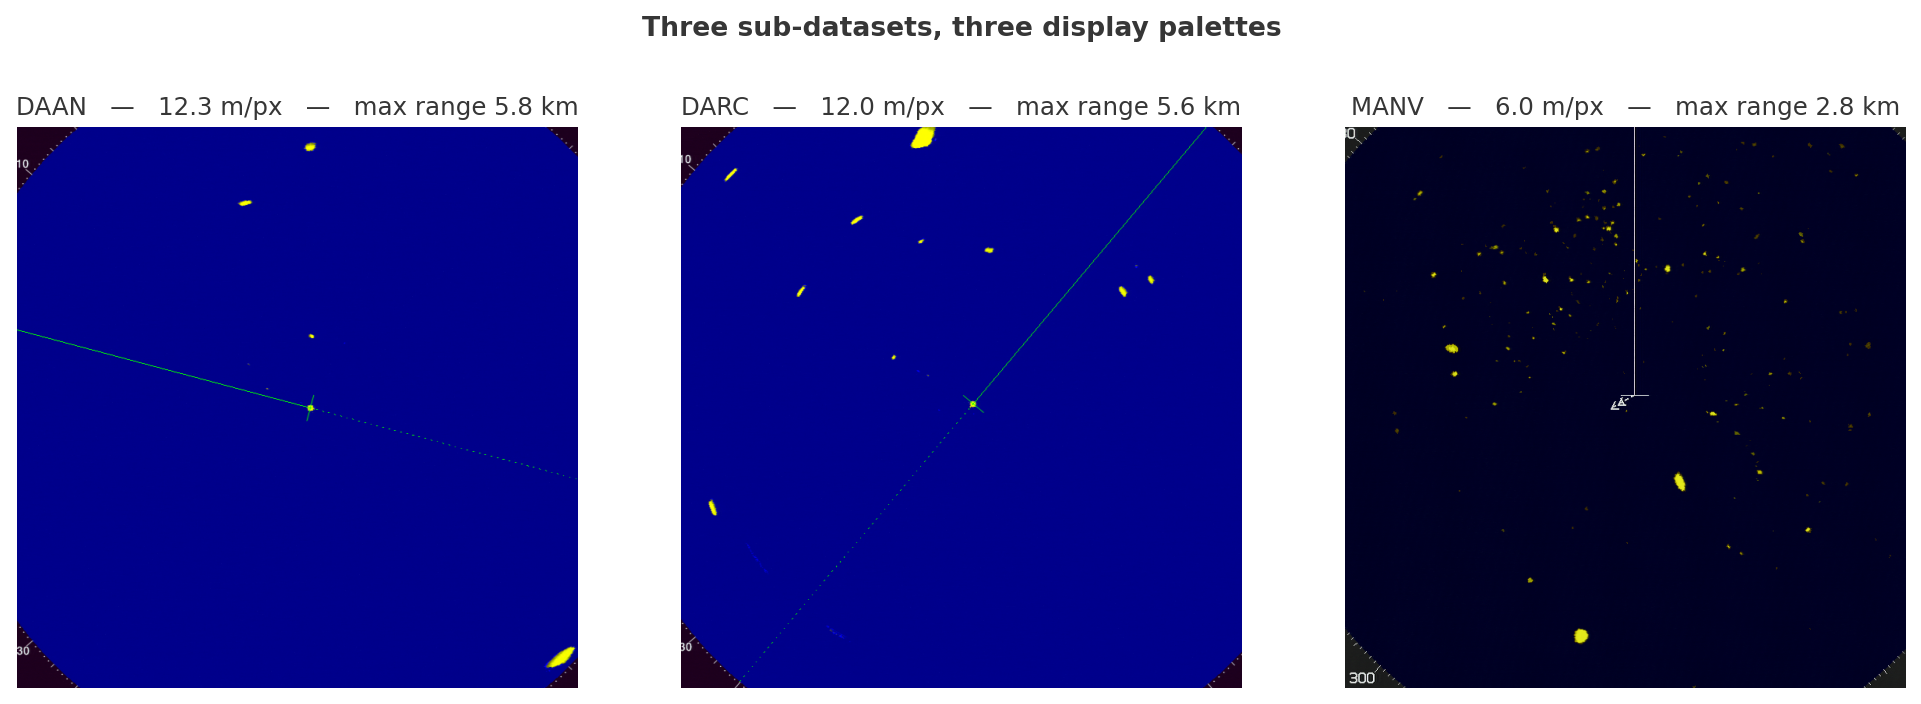
\includegraphics[width=\linewidth]{slide_01_raw_trio.png}
  \end{columns}
  \vspace{0.5em}
  {\tiny\color{black70}April 2026}
\end{frame}

% =======================================================================
% 2 What we are fixing, in one slide
% =======================================================================
\begin{frame}{Why preprocess at all?}
  \begin{columns}[T,onlytextwidth]
    \column{0.54\textwidth}
      \begin{itemize}\setlength\itemsep{0.6em}
        \item DLR ship their ground truth via a default
              \texttt{visualize\_bbox.py}:\\
              polar $\rightarrow$ pixel with $c = (W/2, H/2)$,
              $r_{\max} = 6000$\,m, then\\
              \hl{DBSCAN + 15\,px pad} for the box.
        \item Two systematic issues break this on the released data.
          \begin{itemize}\setlength\itemsep{0.2em}
            \item[\textcolor{garnet}{$\blacksquare$}]
              \hl{Polar origin} is offset $\sim$17\,px from the visual PPI centre.
            \item[\textcolor{garnet}{$\blacksquare$}]
              \hl{MANV range-scale} is 2\,800\,m, \emph{not} 6\,000\,m.
          \end{itemize}
        \item Padded-DBSCAN boxes are \emph{loose} and \emph{off-centre};
              any detector trained / evaluated on them inherits the bias.
      \end{itemize}
    \column{0.42\textwidth}
      \begin{block}{Our pipeline replaces both halves}
        \small
        \textbf{Image side.}\ Per-dataset colour extractor $\rightarrow$
        PPI mask $\rightarrow$ threshold $\rightarrow$ closing $\rightarrow$
        connected components $\rightarrow$ area filter.\\[2pt]
        \textbf{AIS side.}\ Per-dataset polar calibration $\rightarrow$
        DBSCAN seeds in metres $\rightarrow$ tight match against image
        blobs.
      \end{block}
  \end{columns}
\end{frame}

% =======================================================================
% 3 Pipeline at a glance
% =======================================================================
\begin{frame}{Pipeline at a glance}
  \vspace{-0.4em}
  \begin{center}
    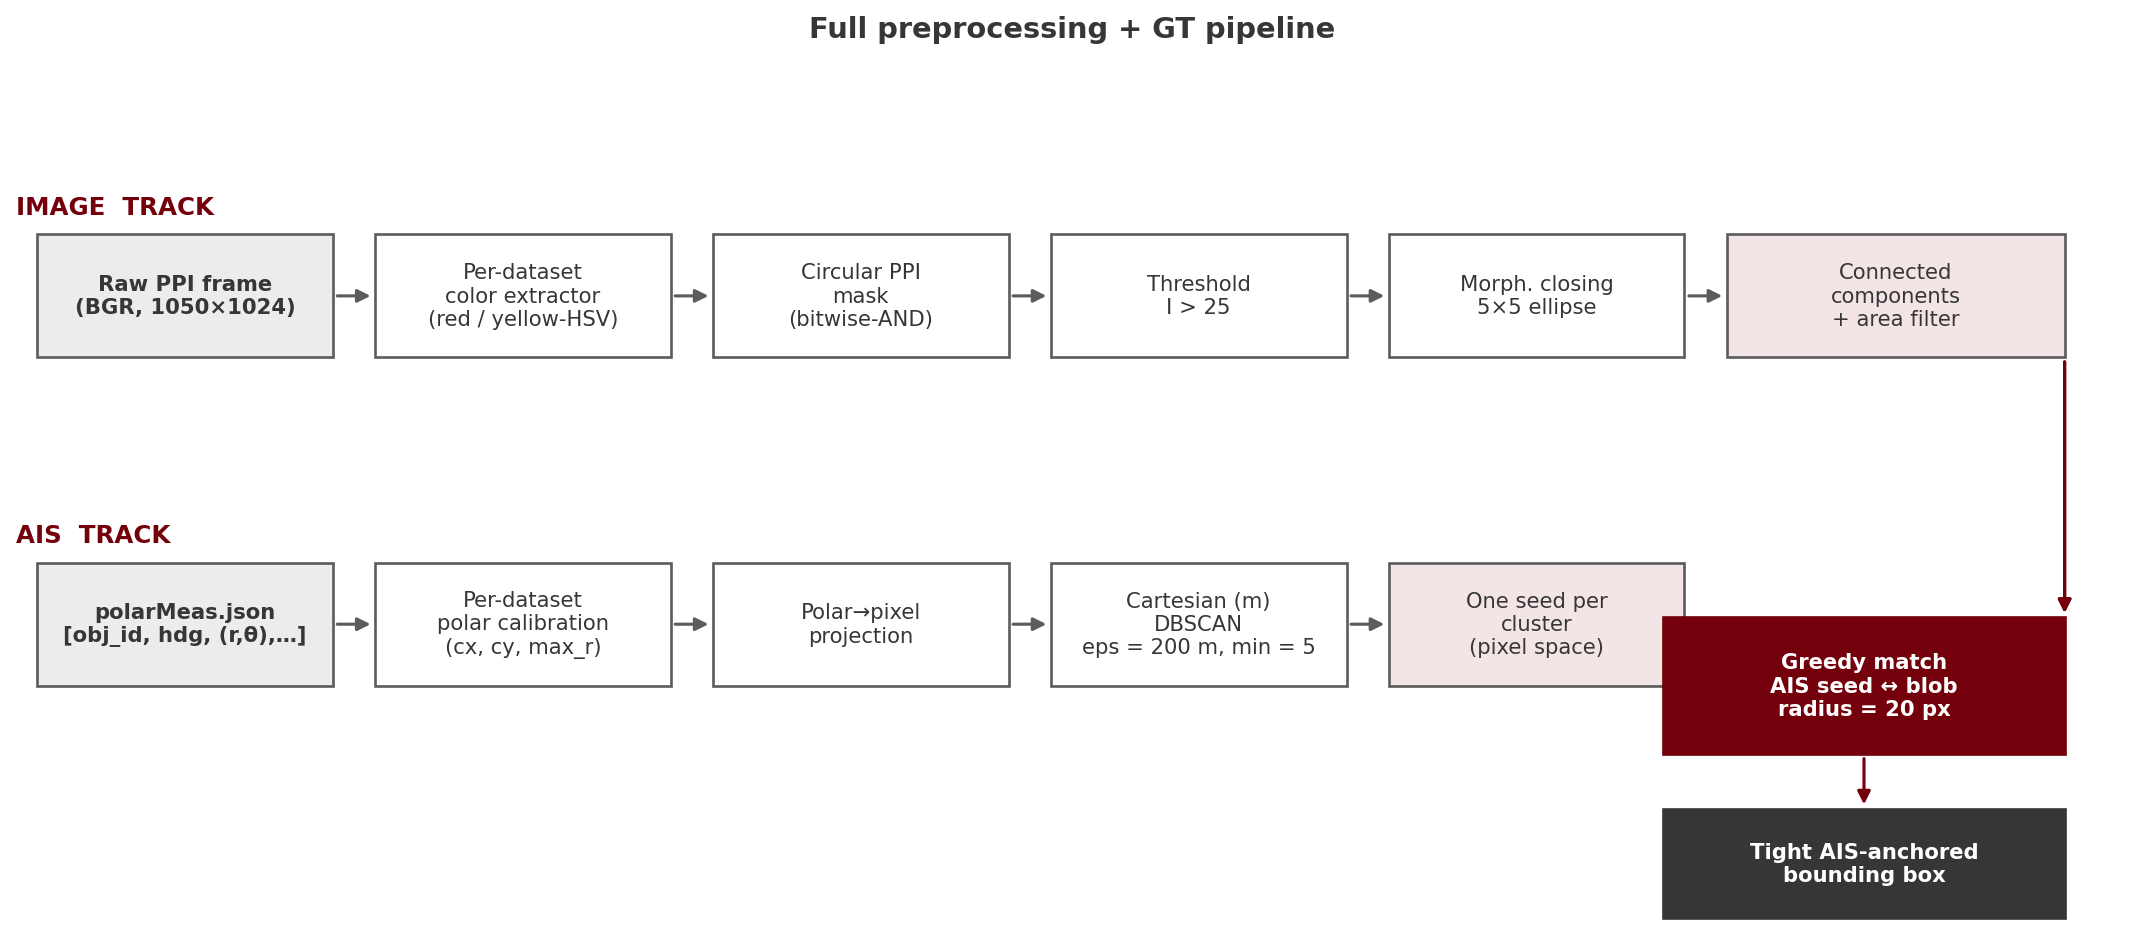
\includegraphics[width=0.96\linewidth]{slide_12_flowchart.png}
  \end{center}
  \vspace{-0.2em}
  \sub{Two independent tracks converge at the greedy matcher. Every
  dataset runs exactly this graph; only the calibration constants
  (colour extractor, $c_x, c_y, r_{\text{max}}$) differ.}
\end{frame}

% =======================================================================
% 4 Three datasets, three palettes
% =======================================================================
\begin{frame}{Input:\ three sub-datasets, three display palettes}
  \begin{center}
    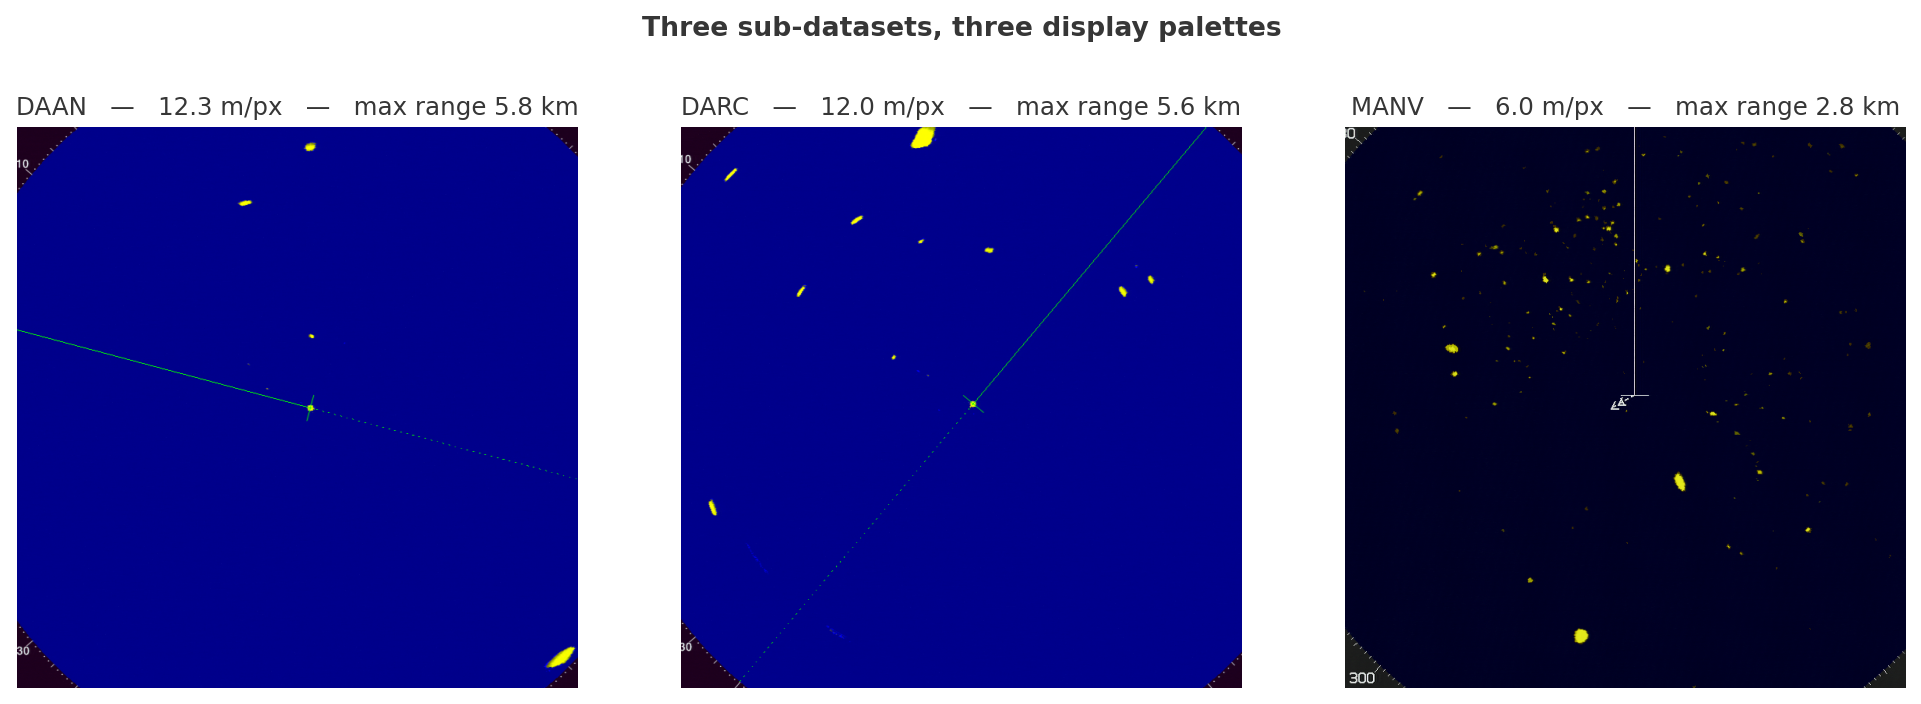
\includegraphics[width=0.95\linewidth]{slide_01_raw_trio.png}
  \end{center}
  \vspace{-0.2em}
  \begin{itemize}\setlength\itemsep{0.15em}
    \item \hl{DAAN / DARC} \sub{open water, $\sim$12\,m/px.}\ \ Solid blue PPI, near-white radar returns, green bearing marks.
    \item \hl{MANV} \sub{harbour manoeuvres, $\sim$6\,m/px.}\ \ Dark near-black PPI, \emph{yellow} radar returns, white UI chrome.
    \item \sub{Every downstream stage must behave differently on MANV than on DAAN/DARC --- starting with which colour channel carries the target signal.}
  \end{itemize}
\end{frame}

% =======================================================================
% 5 Stage 1 — per-dataset colour isolation
% =======================================================================
\begin{frame}{Stage 1 --- per-dataset colour isolation}
  \begin{columns}[T,onlytextwidth]
    \column{0.58\textwidth}
      \centering
      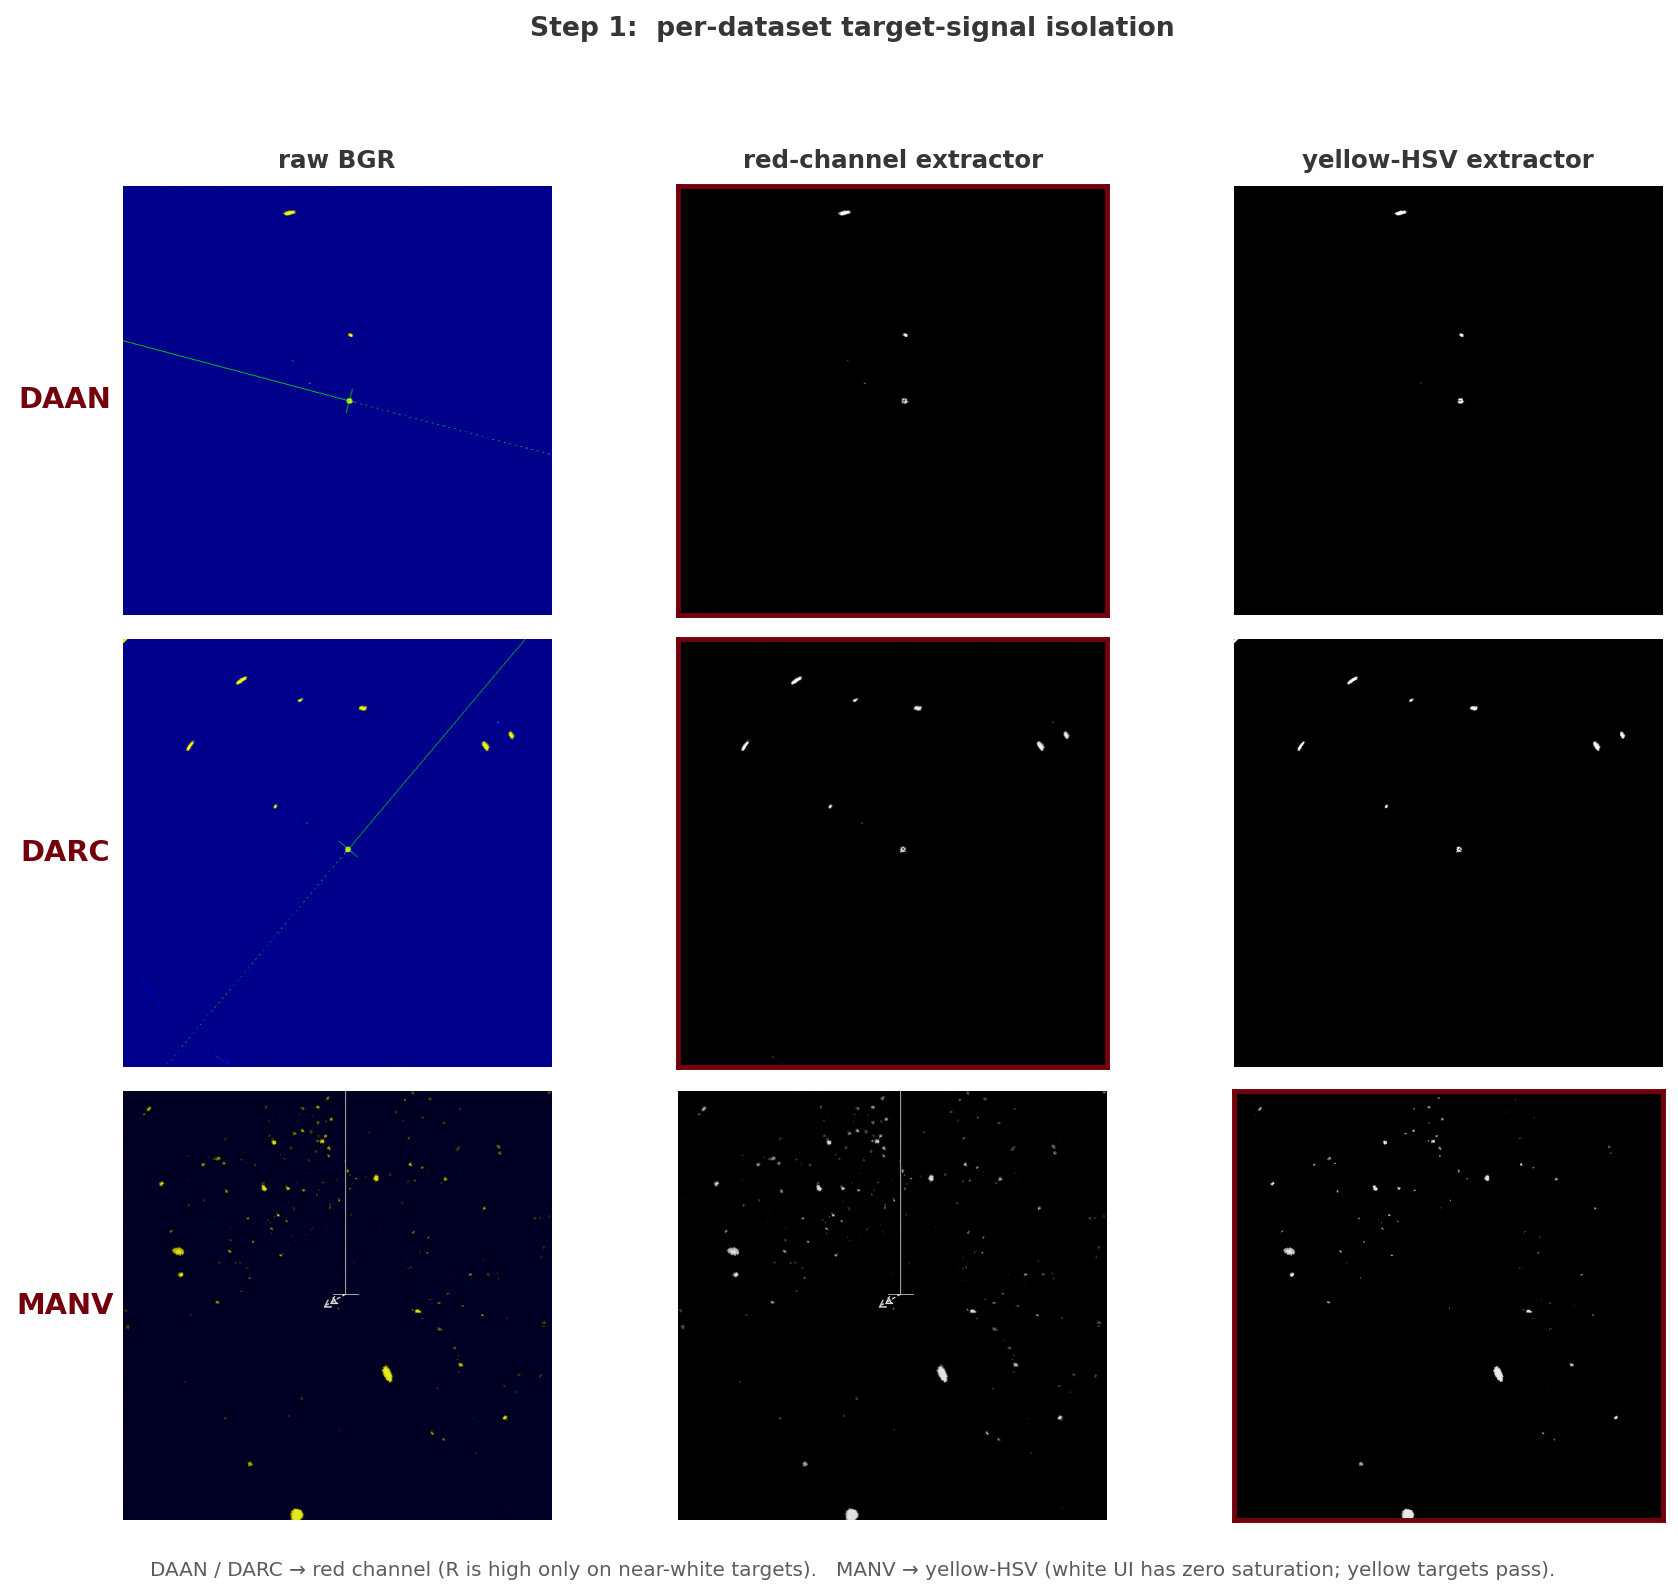
\includegraphics[height=0.82\textheight,keepaspectratio]{slide_02_color_isolation.png}
    \column{0.40\textwidth}
      \footnotesize
      \begin{itemize}\setlength\itemsep{0.4em}
        \item \hl{DAAN / DARC:} red channel. Background B$\approx$140, G$\approx$0, R$\approx$0; green UI has R$=$0; only near-white targets hit R high.
        \item \hl{MANV:} yellow-HSV filter, $H\in[15,50]$, $S\ge80$, $V\ge100$. Red channel would pass white UI chrome; hue\,+\,saturation drops it.
        \item Output: one uint8 signal image per dataset.
      \end{itemize}
      \vspace{0.4em}
      \sub{Garnet border marks the chosen extractor per row.}
  \end{columns}
\end{frame}

% =======================================================================
% 6 Stage 2 — circular PPI mask
% =======================================================================
\begin{frame}{Stage 2 --- circular PPI mask}
  \begin{center}
    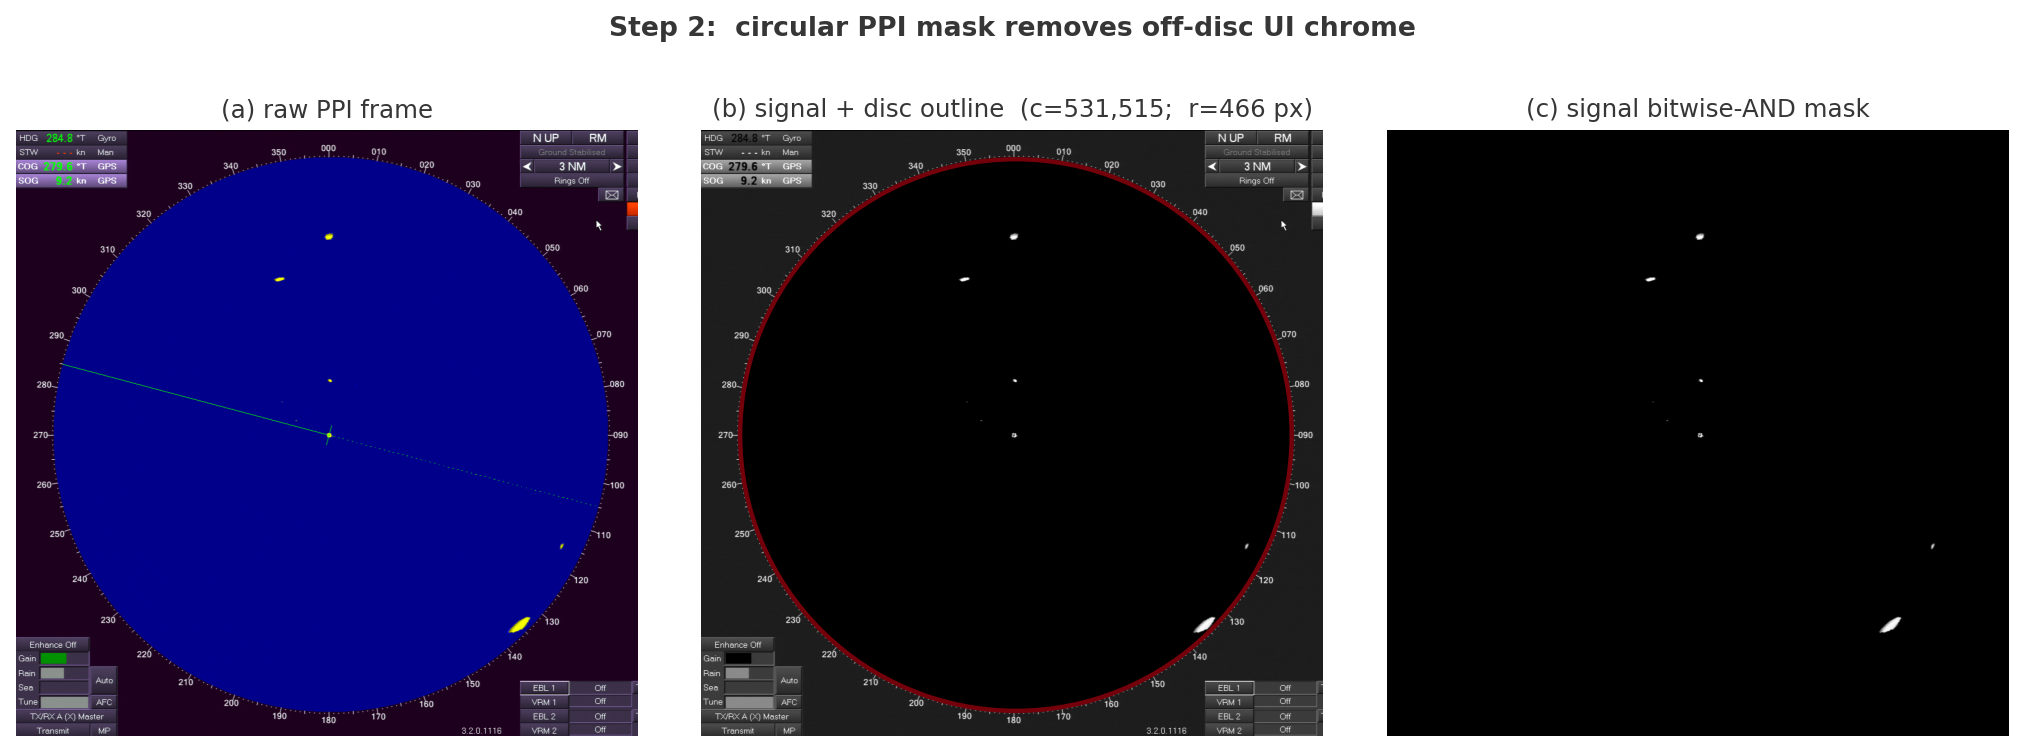
\includegraphics[width=0.88\linewidth]{slide_03_ppi_mask.png}
  \end{center}
  \vspace{-0.4em}
  \footnotesize
  \begin{itemize}\setlength\itemsep{0.1em}
    \item One $1050\times 1024$ binary disc, centre $(531, 515)$, radius $466$\,px; constant across the corpus.
    \item \hl{\texttt{cv2.bitwise\_and}} zeros every off-disc pixel (timestamps, compass ring, scale bar, range rings).
    \item Downstream thresholding and CC labelling see \emph{only} radar returns.
  \end{itemize}
\end{frame}

% =======================================================================
% 7 Stage 3 — threshold + closing
% =======================================================================
\begin{frame}{Stage 3 --- threshold + morphological closing}
  \begin{center}
    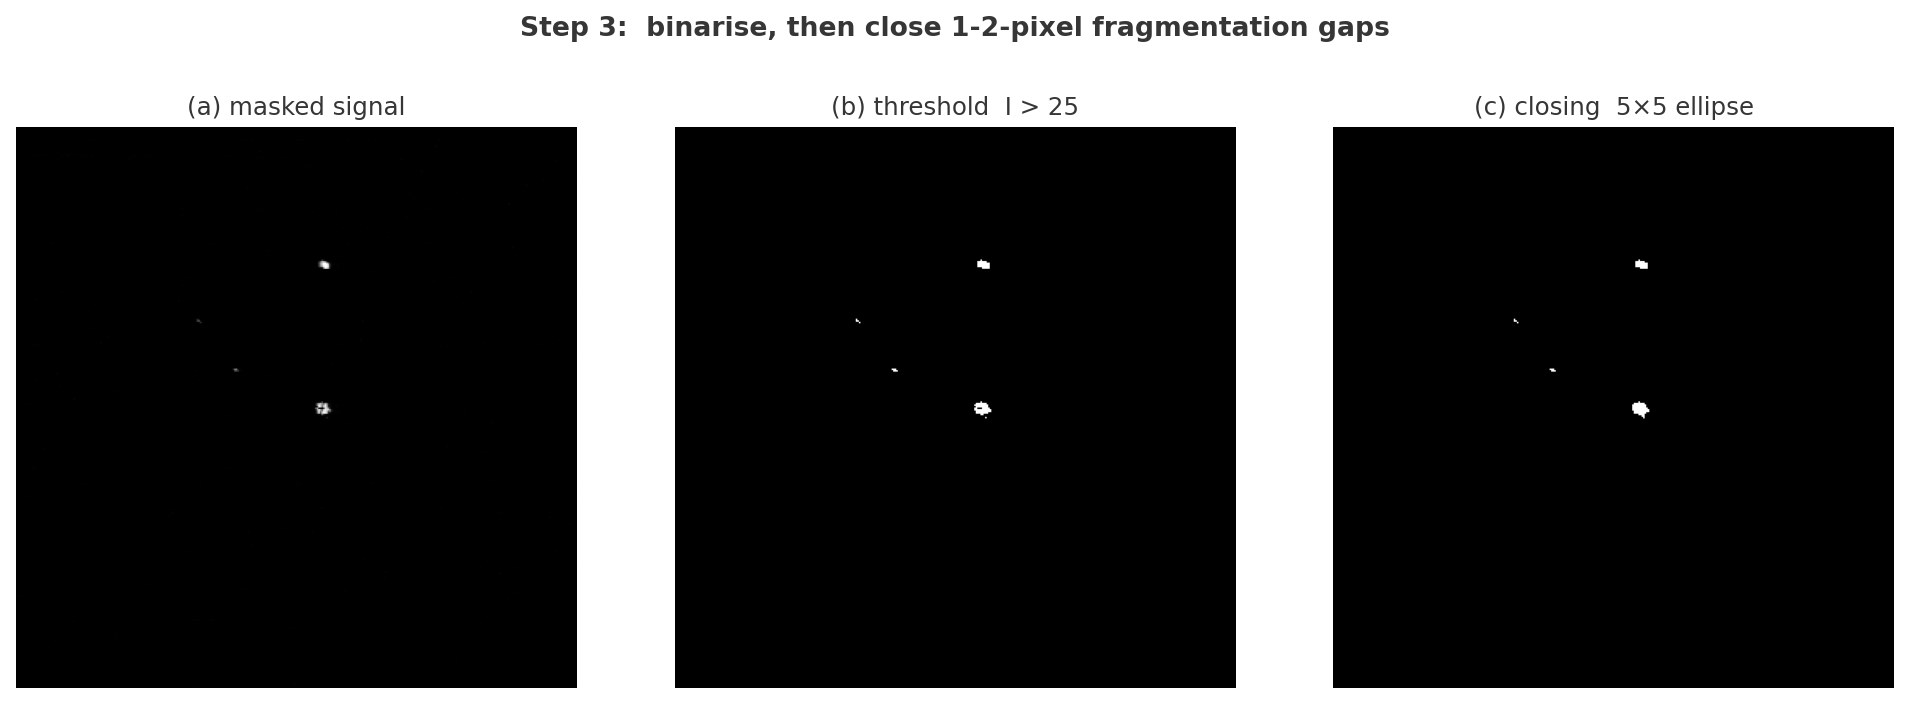
\includegraphics[width=0.86\linewidth]{slide_04_threshold_morph.png}
  \end{center}
  \vspace{-0.4em}
  \footnotesize
  \begin{columns}[T,onlytextwidth]
    \column{0.49\textwidth}
      \begin{itemize}\setlength\itemsep{0.1em}
        \item \hl{Threshold}: $I > 25$ on the masked signal. Same threshold on red-channel (DAAN/DARC) and yellow-HSV-$V$ (MANV) --- both uint8.
      \end{itemize}
    \column{0.49\textwidth}
      \begin{itemize}\setlength\itemsep{0.1em}
        \item \hl{Closing}: $5\times 5$ ellipse, one pass. Bridges 1--2-px gaps inside each return; avoids splitting a ship into many blobs at CC.
      \end{itemize}
  \end{columns}
\end{frame}

% =======================================================================
% 8 Stage 4 — connected components + area filter
% =======================================================================
\begin{frame}{Stage 4 --- connected components + area filter}
  \begin{center}
    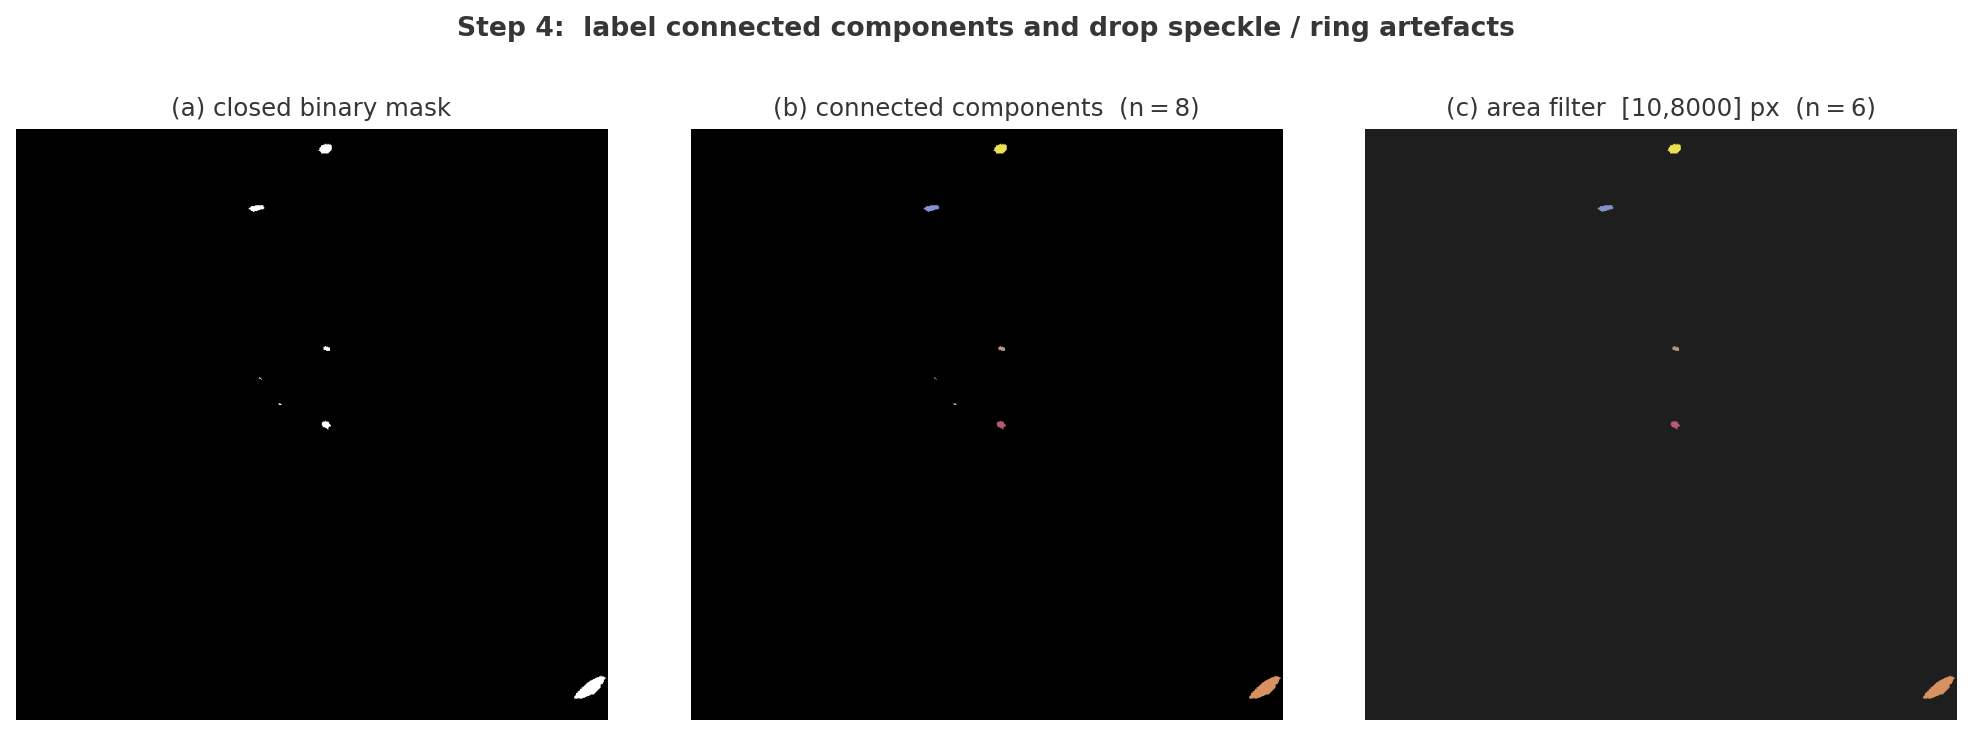
\includegraphics[width=0.90\linewidth]{slide_05_cc_filter.png}
  \end{center}
  \vspace{-0.4em}
  \footnotesize
  \begin{itemize}\setlength\itemsep{0.1em}
    \item \hl{8-connectivity} labelling on the closed mask returns every contiguous bright region --- targets, speckle, and outer-ring artefacts.
    \item \hl{Area filter}: keep $10 \le A \le 8000$\,px. Low bound drops speckle; high bound drops range-ring leakage past the mask.
    \item Each surviving component becomes a candidate blob with $(\text{cx}, \text{cy})$, $(x_1, y_1, x_2, y_2)$, area, peak intensity.
  \end{itemize}
\end{frame}

% =======================================================================
% 9 The DLR projection bug (before we fix it)
% =======================================================================
\begin{frame}{The DLR default polar projection is wrong on MANV}
  \begin{columns}[T,onlytextwidth]
    \column{0.62\textwidth}
      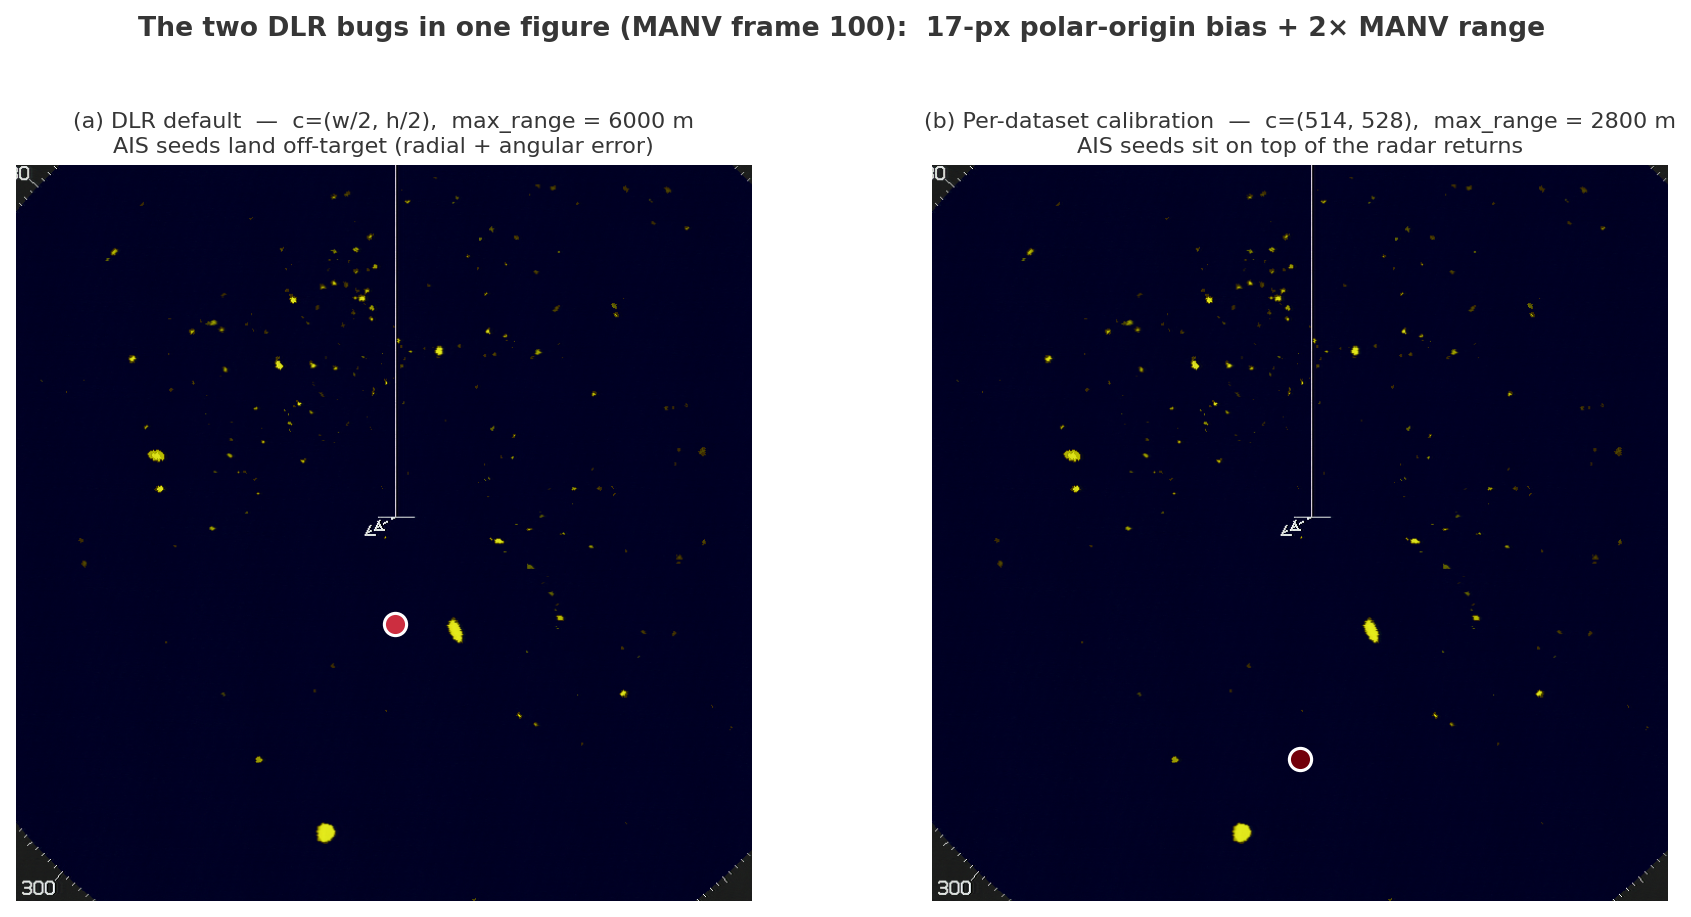
\includegraphics[width=\linewidth]{slide_06_polar_bias.png}
    \column{0.36\textwidth}
      \begin{itemize}\setlength\itemsep{0.45em}
        \item DLR default uses $(c_x, c_y) = (W/2, H/2)$ and
              $r_{\max} = 6000$\,m \hl{for all three sub-datasets}.
        \item On MANV this places AIS seeds \hl{40--70\,px} from the
              actual radar blobs.
        \item Two errors stack: the polar origin is off by $\sim$17\,px
              \emph{and} MANV's range is half what DLR's script assumes.
        \item On DAAN / DARC the range is correct; only the 17-px bias
              remains, still large enough to break the AIS$\rightarrow$
              blob match inside a 20-px radius.
      \end{itemize}
  \end{columns}
\end{frame}

% =======================================================================
% 10 Per-dataset calibration
% =======================================================================
\begin{frame}{Per-dataset calibration fixes both errors}
  \begin{center}
    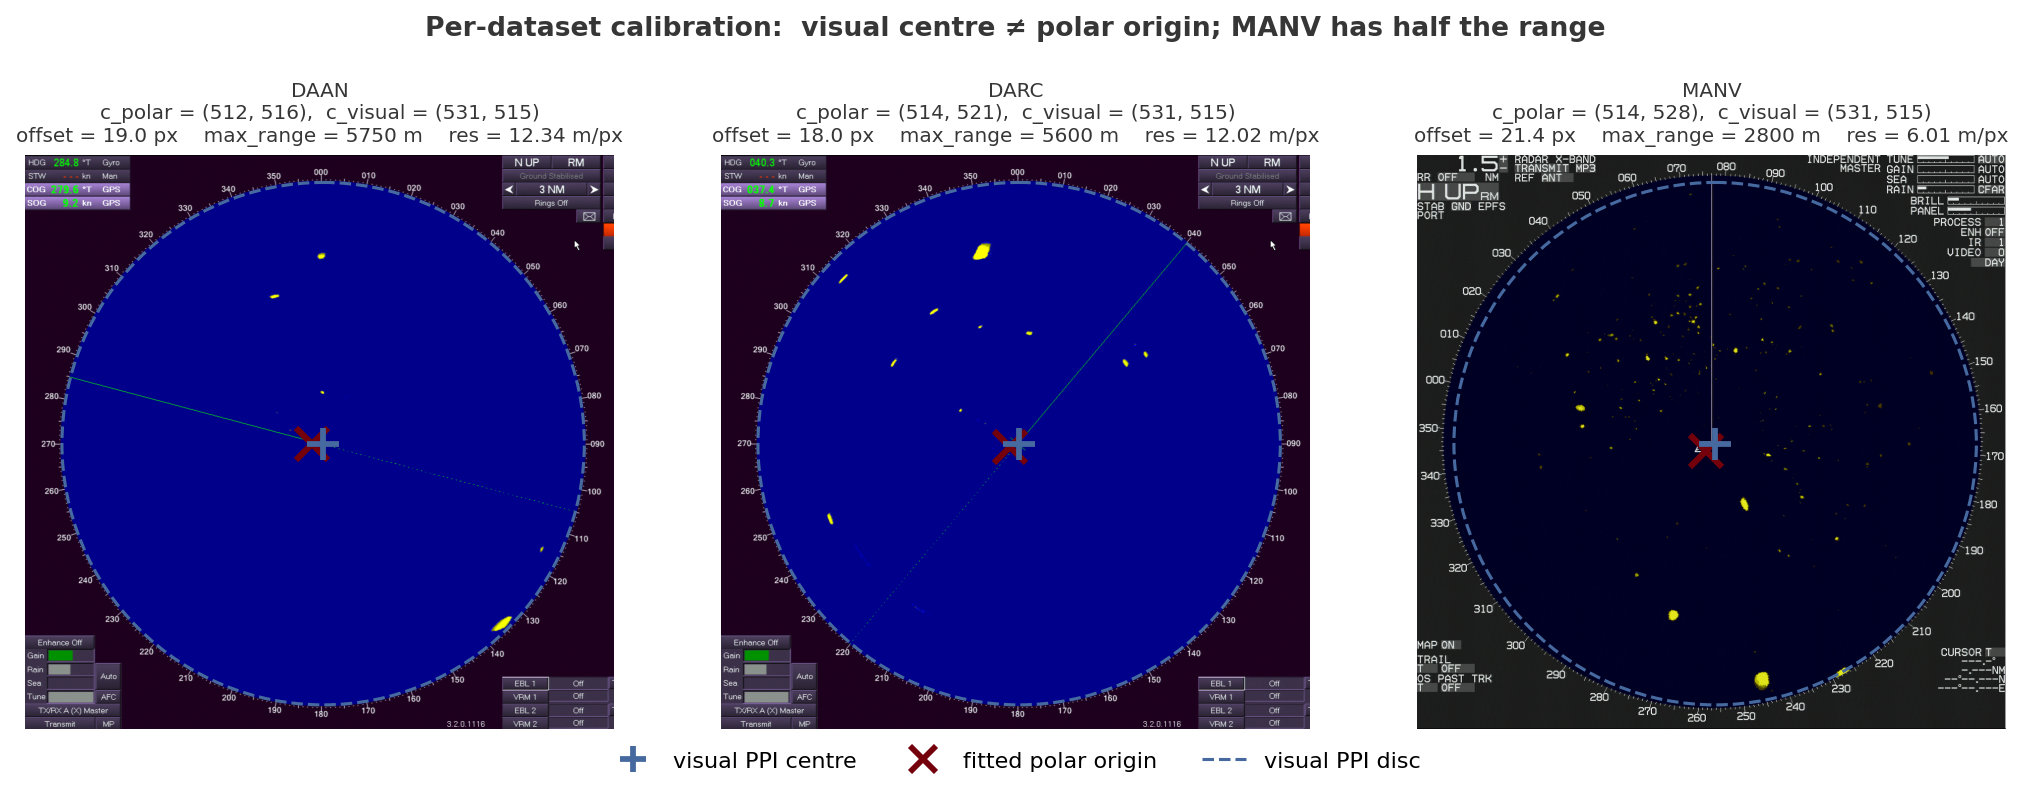
\includegraphics[width=0.86\linewidth]{slide_07_calibration_schematic.png}
  \end{center}
  \vspace{-0.5em}
  \begin{columns}[T,onlytextwidth]
    \column{0.49\textwidth}
      \scriptsize
      \begin{tabular}{@{}l r r r r@{}}
        \toprule
        \textbf{Sub-dataset} & $c_x$ & $c_y$ & $r_{\max}$\,[m] & res\,[m/px] \\
        \midrule
        DAAN & 512 & 516 & 5\,750 & 12.34 \\
        DARC & 514 & 521 & 5\,600 & 12.02 \\
        MANV & 514 & 528 & 2\,800 & \phantom{0}6.01 \\
        \bottomrule
      \end{tabular}
    \column{0.49\textwidth}
      \footnotesize
      $r_{\text{px}} = (r / r_{\max}) \cdot r_{\text{px,max}}$;\ \ $p_x = c_x + r_{\text{px}}\sin\theta$;\ \ $p_y = c_y - r_{\text{px}}\cos\theta$.\\[2pt]
      Residuals after calibration drop to \hl{5--7\,px median} (shown later).
  \end{columns}
\end{frame}

% =======================================================================
% 11 Stage 5 — AIS DBSCAN seed splitting
% =======================================================================
\begin{frame}{Stage 5 --- AIS\,$\rightarrow$\,seed DBSCAN splitting}
  \begin{center}
    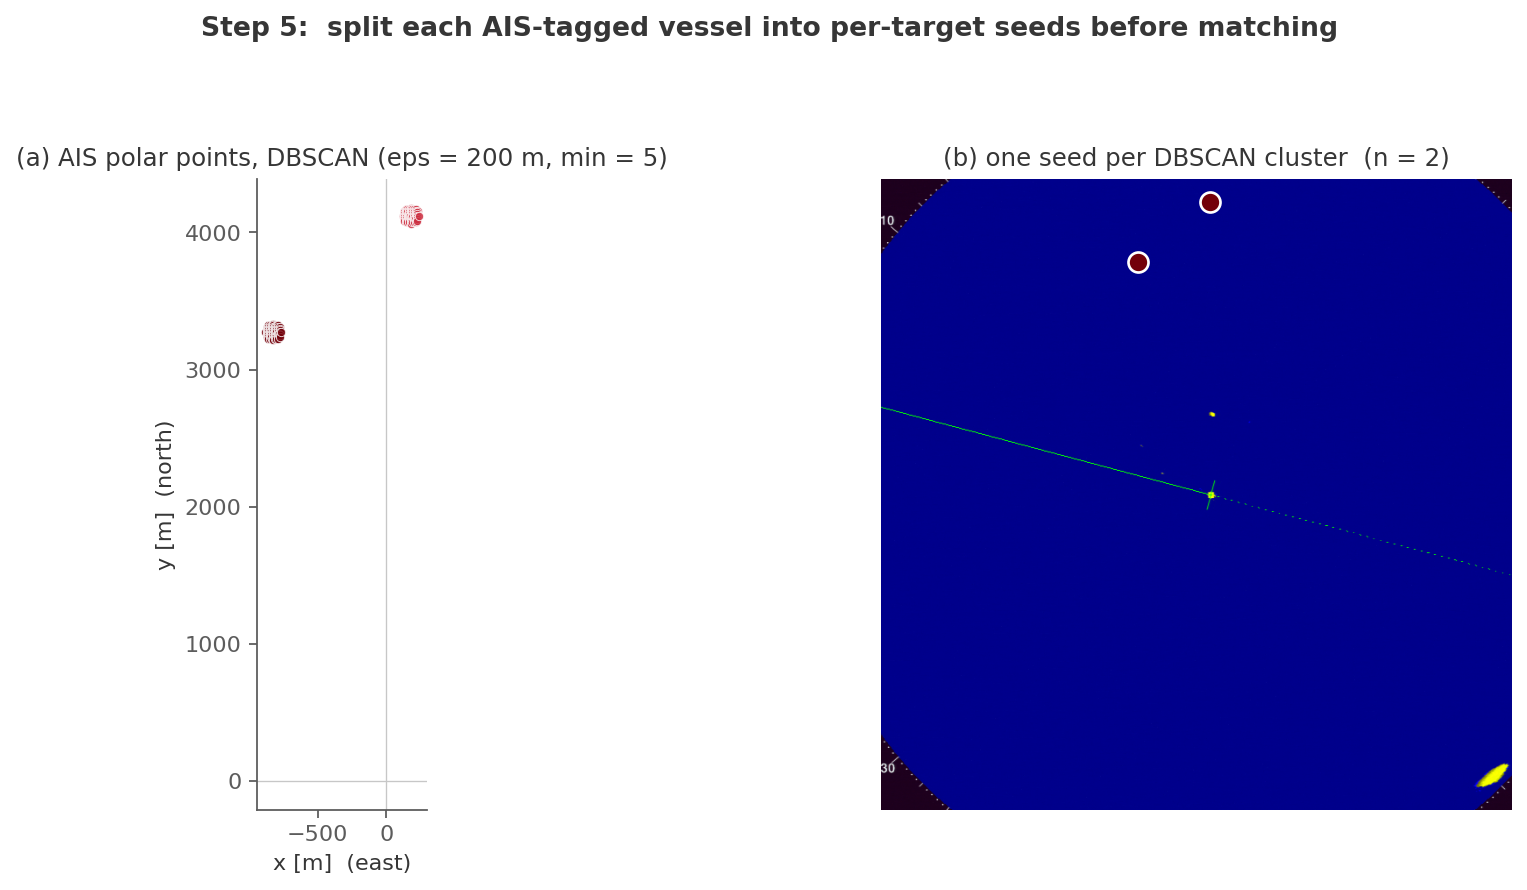
\includegraphics[height=0.72\textheight,keepaspectratio]{slide_08_dbscan_seeds.png}
  \end{center}
  \vspace{-0.3em}
  \footnotesize
  \begin{itemize}\setlength\itemsep{0.1em}
    \item An AIS record reports many polar points per vessel; multiple vessels can share one record in the release.
    \item \hl{DBSCAN in Cartesian metres} ($\varepsilon = 200$\,m, min $= 5$) splits each AIS object into per-target clusters.
    \item Each cluster collapses to one pixel-space seed via the calibrated projection.
  \end{itemize}
\end{frame}

% =======================================================================
% 12 Stage 6 — greedy match
% =======================================================================
\begin{frame}{Stage 6 --- greedy AIS\,$\leftrightarrow$\,blob matching}
  \begin{center}
    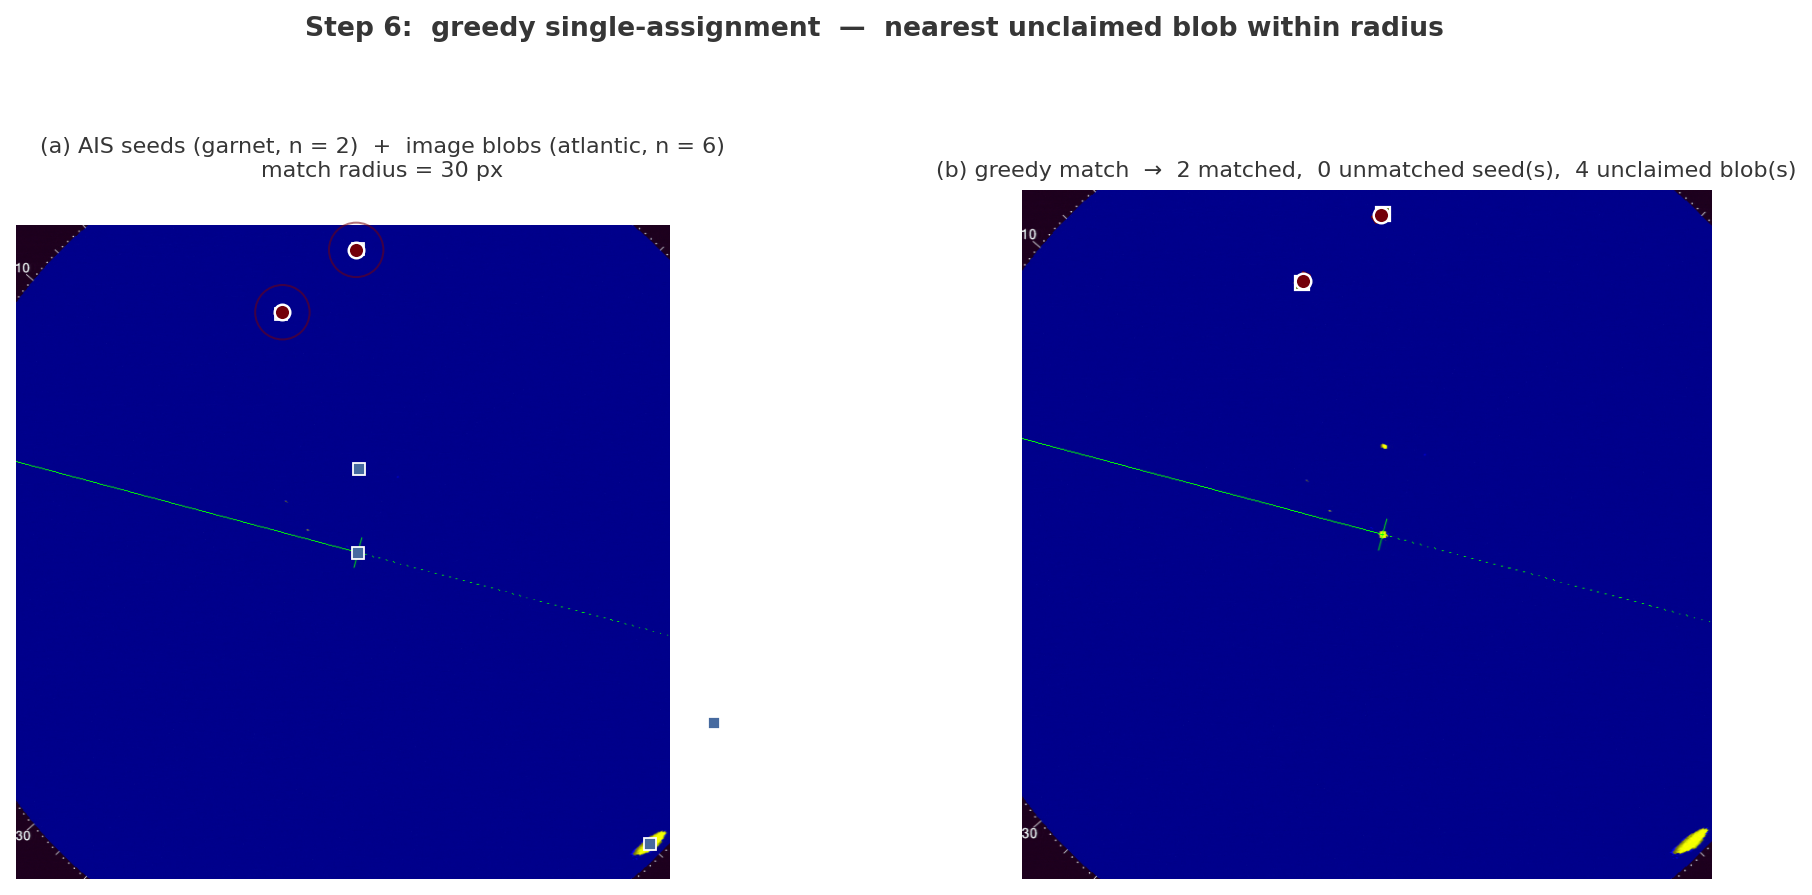
\includegraphics[height=0.72\textheight,keepaspectratio]{slide_09_greedy_match.png}
  \end{center}
  \vspace{-0.3em}
  \footnotesize
  \begin{itemize}\setlength\itemsep{0.1em}
    \item Seeds ordered by AIS point-count descending --- the most confident AIS track picks first.
    \item Each seed claims the \hl{nearest unclaimed blob within 20\,px}; greedy, one-to-one.
    \item Unmatched seeds (warm grey) and unclaimed blobs are tracked for diagnostics, never silently merged.
  \end{itemize}
\end{frame}

% =======================================================================
% 13 Result: our boxes vs DLR-default boxes
% =======================================================================
\begin{frame}{Result --- DLR default vs AIS-anchored, all three datasets}
  \begin{columns}[T,onlytextwidth]
    \column{0.48\textwidth}
      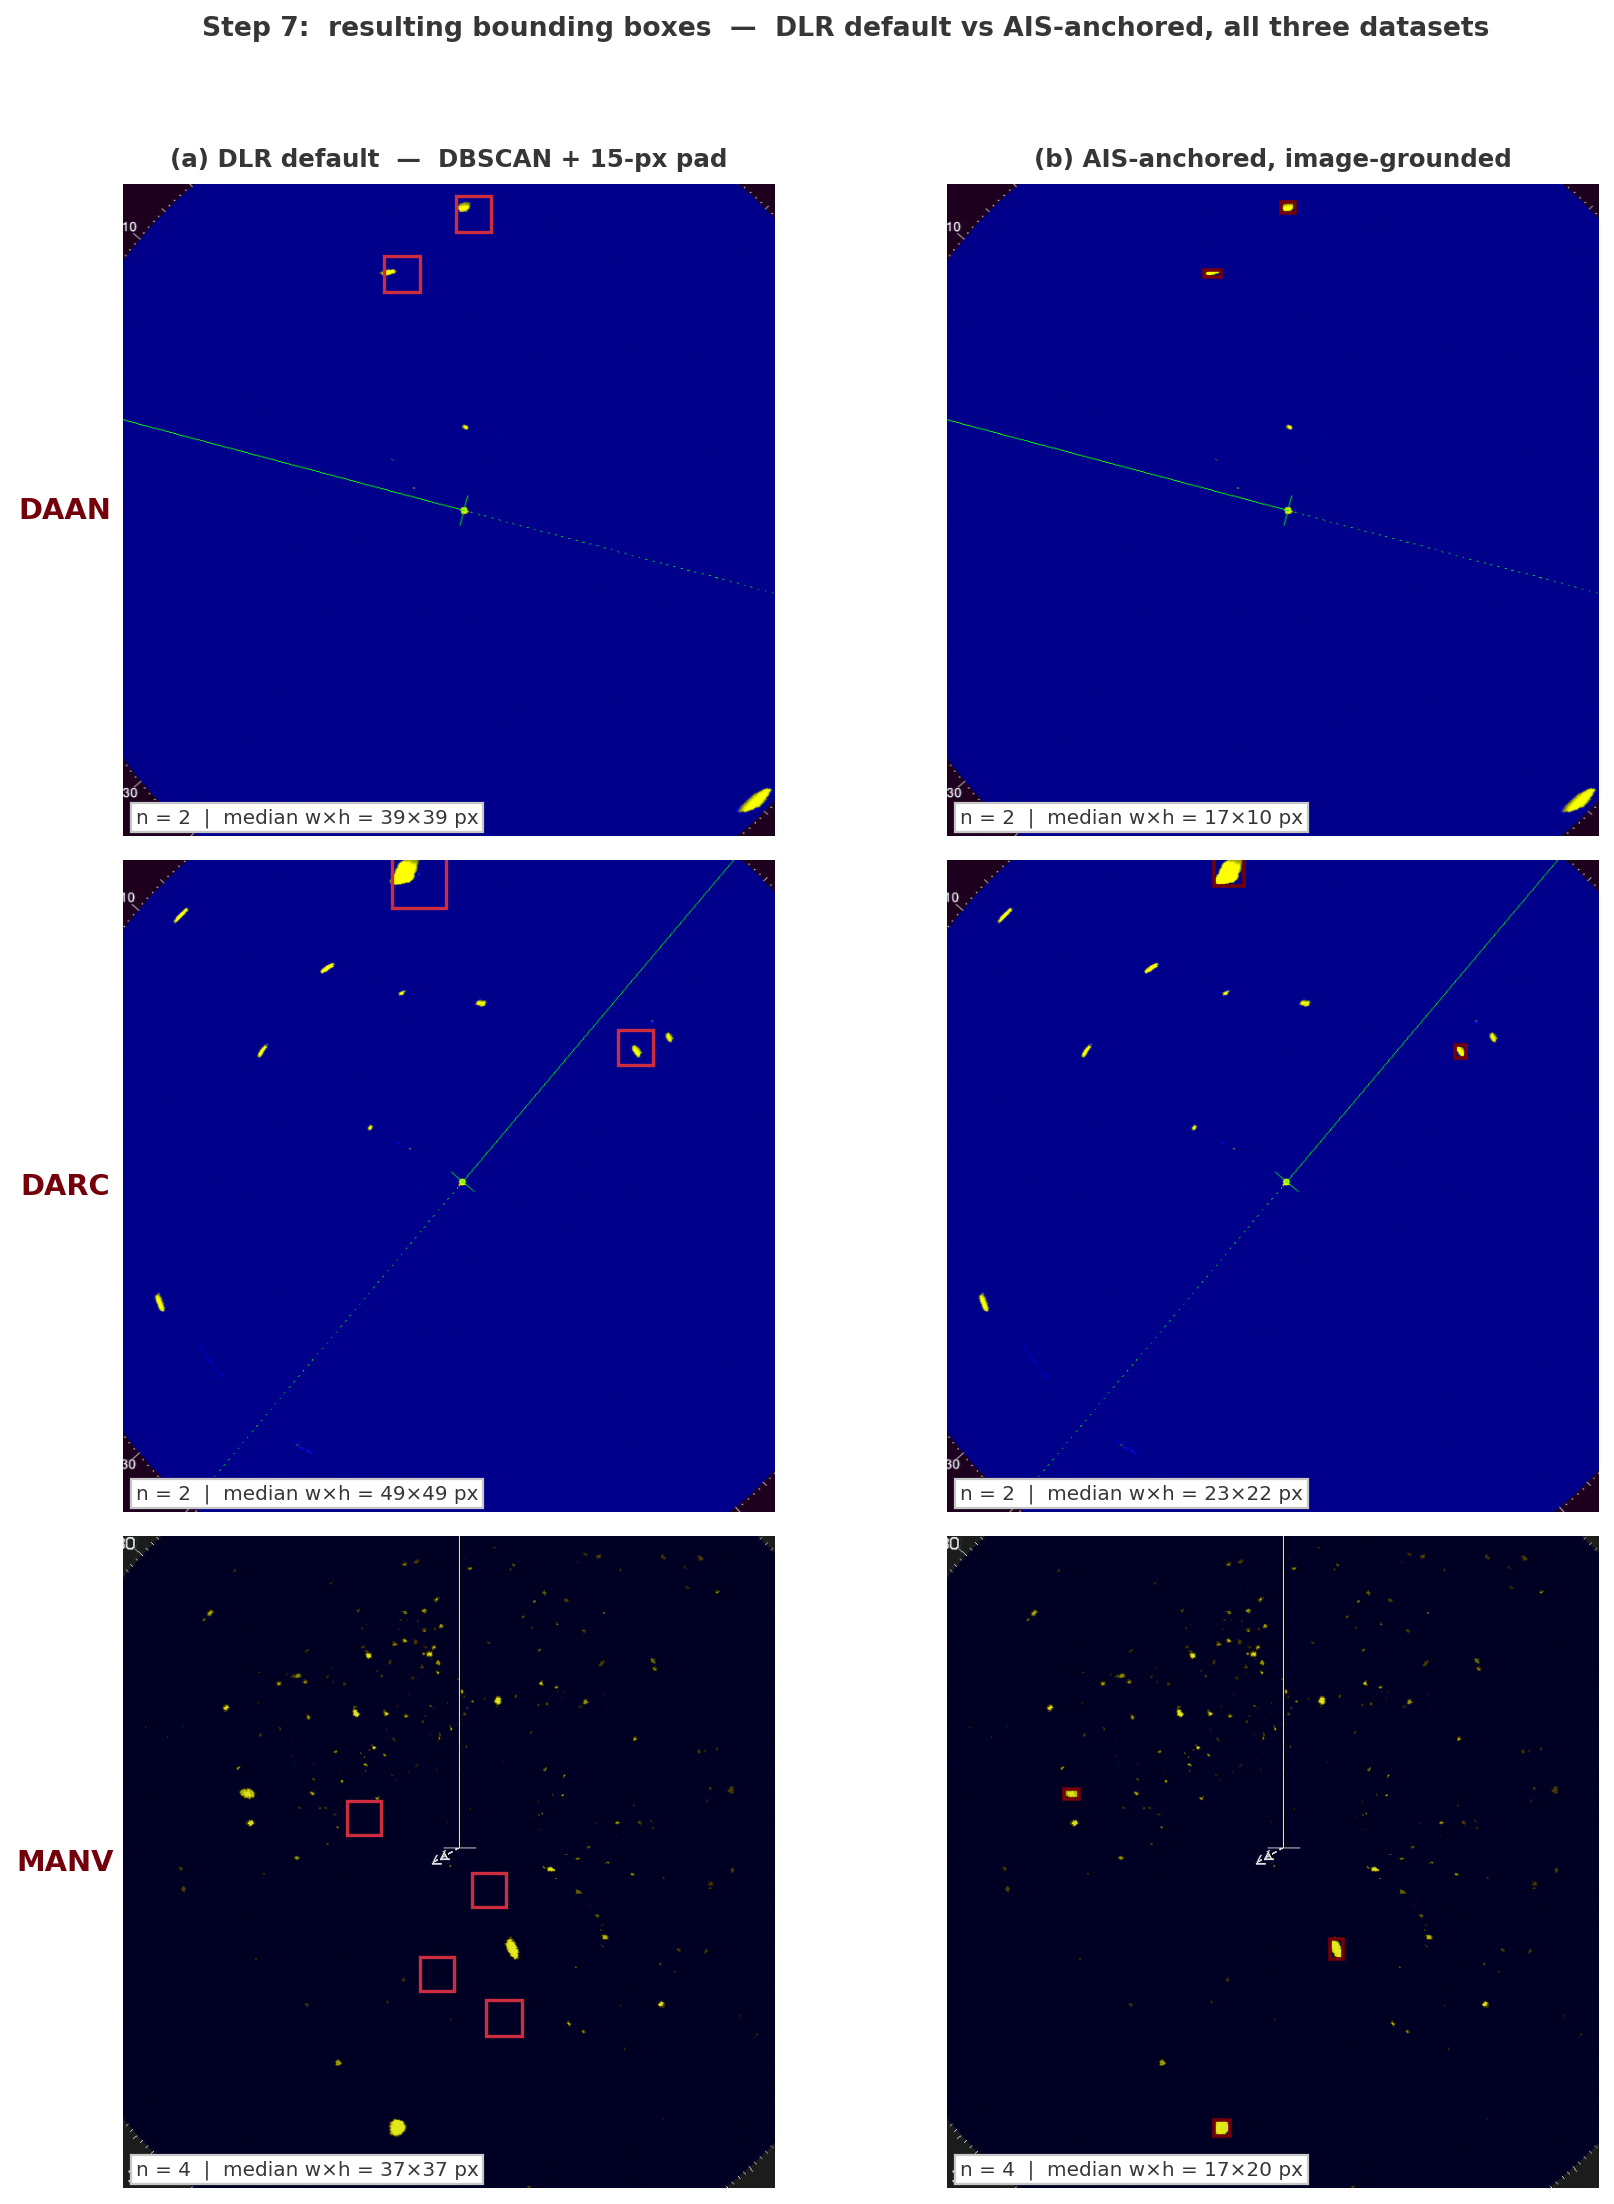
\includegraphics[height=0.82\textheight,keepaspectratio]{slide_10_box_comparison_trio.png}
    \column{0.50\textwidth}
      \footnotesize
      \begin{itemize}\setlength\itemsep{0.4em}
        \item \textcolor{rose}{\textbf{Rose}} --- DLR default (DBSCAN $+$ 15-px pad). Boxes float a few pixels off the signal and are padded to $\sim$33\,px regardless of target size.
        \item \hl{Garnet} --- AIS-anchored, image-grounded. Boxes come from the connected-component extent of the \emph{matched} blob --- tight by construction.
        \item Every sub-dataset sees the same qualitative improvement; the effect is strongest on MANV where both bugs compound.
      \end{itemize}
  \end{columns}
\end{frame}

% =======================================================================
% 14 Residual histogram — calibration validation
% =======================================================================
\begin{frame}{Calibration validation:\ AIS-seed $\rightarrow$ nearest-blob residual}
  \begin{center}
    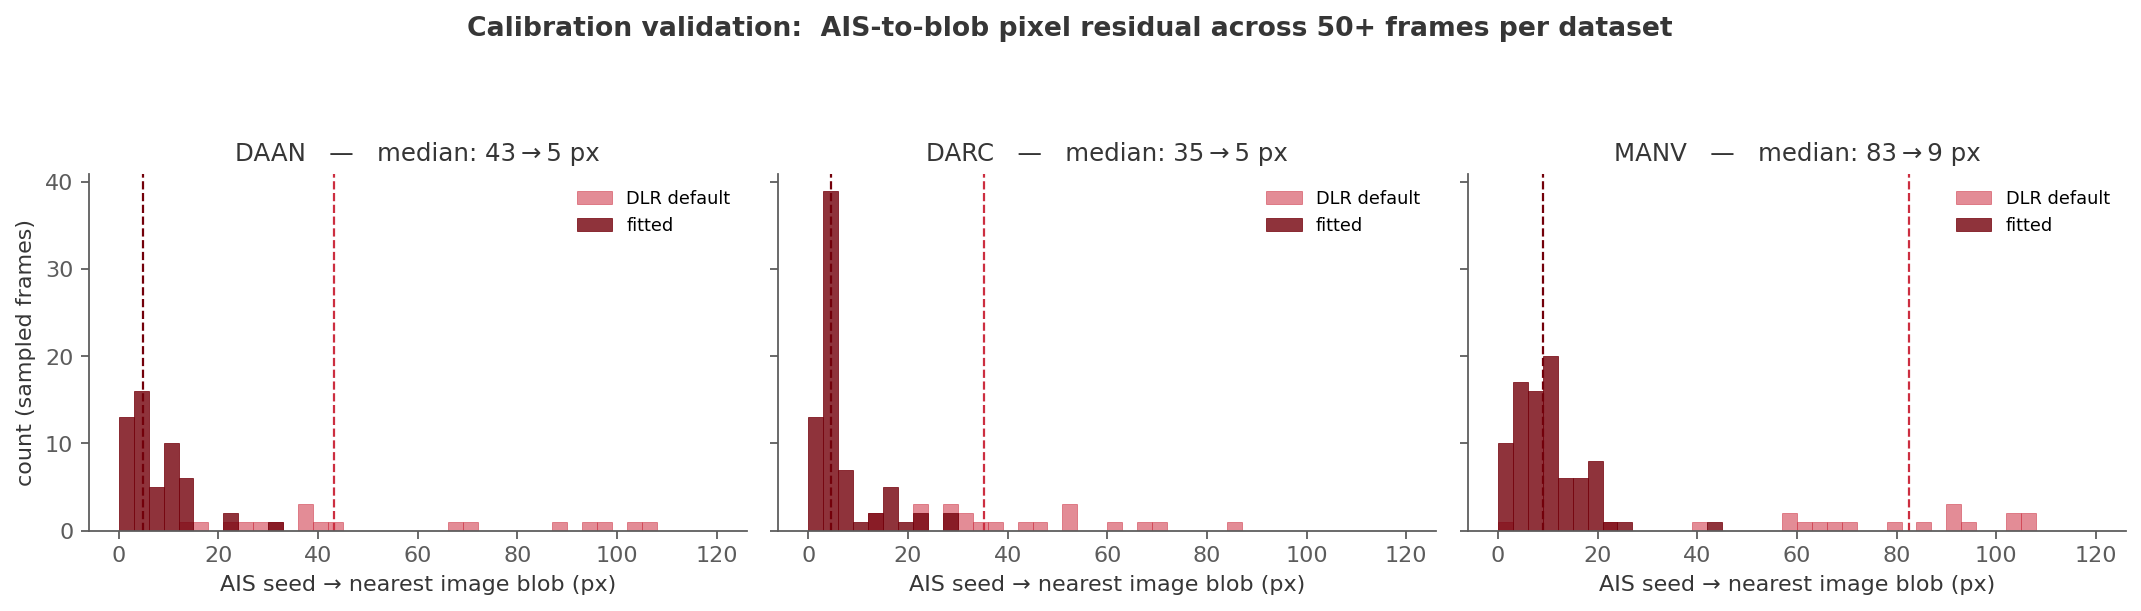
\includegraphics[width=0.92\linewidth]{slide_11_residual_hist.png}
  \end{center}
  \vspace{-0.4em}
  \footnotesize
  \begin{itemize}\setlength\itemsep{0.1em}
    \item \hl{DAAN / DARC}: median residual drops from $\sim$22\,px to $\sim$5\,px.
    \item \hl{MANV}: median residual drops from $\sim$67\,px to $\sim$7\,px --- the $2\times$ range fix alone shrinks the right tail by half.
    \item Measured across $\sim$50 sampled frames per sub-dataset --- the fix is not a one-frame fluke.
  \end{itemize}
\end{frame}

% =======================================================================
% 15 Summary
% =======================================================================
\begin{frame}{Summary --- what preprocessing actually gave us}
  \small
  \begin{itemize}\setlength\itemsep{0.35em}
    \item \hl{One pipeline, three datasets.}\ Per-dataset colour extractor + per-dataset polar calibration; everything else is shared.
    \item \hl{Two documented DLR bugs corrected.}\ 17-px polar-origin bias and $2\times$ MANV range-scale. Median AIS$\rightarrow$blob residual drops from 22--67\,px to 5--7\,px.
    \item \hl{Bounding boxes are now image-grounded and tight.}\ Connected-component extents of the matched radar return replace DBSCAN-padded $\sim$33$\times$33 boxes.
    \item Every classical and deep detector in the final benchmark is evaluated against \emph{this} ground truth --- a necessary condition for comparability across methods and datasets.
  \end{itemize}
  \vspace{0.2em}
  \begin{center}
    {\color{garnet}\rule{0.8\textwidth}{0.6pt}}\par
    \vspace{0.2em}
    \footnotesize Pipeline code:\ \texttt{preprocessing\_report/\{radar\_mask,ais\_anchored\_gt\}.py}\\
    \footnotesize Figures reproducible via \texttt{generate\_slides\_figures.py}.
  \end{center}
\end{frame}

\end{document}
